\ifx\XeTeXversion\undefined\pdfoutput=1\fi % pdfLaTeX (arXiv); skipped under XeTeX
\documentclass[10pt]{article}
\usepackage{tmlr}
% For the camera-ready version: \usepackage[accepted]{tmlr}
\usepackage{microtype}
\usepackage{amsmath,amssymb,amsthm}
\usepackage{booktabs}
\usepackage{array}
\usepackage{graphicx}
\usepackage{xcolor}
\usepackage{enumitem}
\usepackage[colorlinks=true,linkcolor=blue!60!black,citecolor=blue!60!black,urlcolor=blue!60!black]{hyperref}

\newtheorem{theorem}{Theorem}
\newtheorem{proposition}{Proposition}
\newtheorem{corollary}{Corollary}
\theoremstyle{definition}
\newtheorem{definition}{Definition}
\newtheorem{numresult}{Numerical result}
\theoremstyle{remark}
\newtheorem*{remark}{Remark}

\newcommand{\lam}{\lambda}
\DeclareMathOperator{\logit}{logit}
\setlist{itemsep=1pt,topsep=3pt}

\title{\textbf{Equilibrium or Retrieval?}\\[2pt]
\large Do LLM Agents Derive or Recall Game-Theoretic Equilibria,\\
and What That Means for Mechanism Design}
\author{\name Anonymous}


\begin{document}
\maketitle

\begin{abstract}
Large language models (LLMs) play textbook games well, but a model can reach the textbook answer
in two ways: by deriving it from the rules, or by recognising a famous game and recalling its
answer. We separate the two with \emph{isomorphic twins}. Each question is asked in its standard
wording and in disguised wordings with identical numbers, rules and information but no game
vocabulary, and every answer is paired with a competence check in the same wording. In four
pre-registered studies, four models from four developers answer 20{,}368 questions about a Vickrey
auction, a Cournot duopoly, a finitely repeated prisoner's dilemma and a public goods game. The
answer differs by model. Two models solve a Cournot game they no longer recognise and are not
fooled by traps that make the textbook answer wrong. A third loses the equilibrium step by step
as recognition falls, and gives the textbook answer about five times as often in its standard wording. A
fourth loses it as soon as the game's familiar vocabulary goes. In the prisoner's dilemma, recognition retrieves
a script of cooperation rather than the equilibrium, and logit quantal response equilibrium
(QRE) fails pre-registered calibration for every model. We then derive mechanisms for QRE
agents, including a closed-form cooperation subsidy, and prove a ceiling: below the subsidy's
halfway point, no regular QRE produces cooperation above one half, at any precision. In a
pre-registered test, the subsidy derived from fitted QRE reaches its target in every model but
overpays by up to twenty times, and classical theory predicts the response better. The low fitted
precision reflected cooperation that QRE cannot represent, not insensitivity to incentives.
\end{abstract}


% =====================================================================================
\section{Introduction}

LLM agents are beginning to act in settings that game theory was built to analyse: bidding in
auctions, setting prices, negotiating, and drawing on shared resources. The rules of such
settings are designed, and designing them, which is the business of mechanism design, requires a
model of how participants behave. Classical mechanism design assumes rational players who
best-respond. Behavioural mechanism design replaces them with an empirically fitted model, most
prominently the logit quantal response equilibrium (QRE) \citep{mckelvey1995qre,goeree2016qre},
in which players choose better actions more often than worse ones, with a precision $\lam$.

Before a fitted model of LLM play can be trusted to design anything, a prior question must be
settled: \emph{is the play we measure reasoning about the rules in front of the model, or
retrieval of answers to famous problems?} The concern is concrete. The Vickrey auction, the
Cournot duopoly, the prisoner's dilemma and the public goods game are among the most
written-about games in any corpus a model is trained on. ``Bid your true value'',
``produce $(a-c)/3b$'' and ``defect in the last round'' appear thousands of times. LLM accuracy is
known to depend on how familiar a task looks, not only on what it requires
\citep{mccoy2024embers}. A mechanism tuned to recalled play may fail precisely when the designer
changes the rules, which is the only reason to design a mechanism at all.

\paragraph{Approach.} We hold each game fixed and vary only its \emph{wording}:
\begin{enumerate}[label=(\roman*)]
\item \textbf{Isomorphic twins.} The disguised wording preserves every number, rule and
  information structure, and removes the game's vocabulary. An extreme disguise (Stage~2C)
  removes the story too, codes the answer (for example, ``your offer is $3x+5$'') and replaces
  the answer box. Section~\ref{sec:framework} shows that a purely deriving agent's play is
  invariant to such relabelling, so any wording effect rejects pure derivation.
\item \textbf{Competence probes.} A short calculation in the same wording follows every answer.
  Only answers whose probe is passed are analysed, so a wording effect cannot be a reading
  failure.
\item \textbf{Measured recognition.} A validated code records whether the model's reasoning
  names the game (agreement with blind hand coding $\kappa = 1.00$). Recognition and play are
  then read jointly, by rules fixed before the data.
\item \textbf{Pre-registration.} Four registrations on OSF fix the predictions, sample sizes,
  exclusions and tests before each study \citep{nosek2018prereg}. The analysis code was locked
  by cryptographic fingerprint.
\end{enumerate}

\paragraph{Findings.}
\begin{itemize}
\item \textbf{Derive or recall differs by model.} Nemotron and Kimi solve a Cournot game they no
  longer recognise. gpt-oss's play tracks recognition across three wordings. Gemini loses the
  Cournot equilibrium as soon as the game's familiar vocabulary goes.
\item \textbf{Traps confirm the split.} When one rule makes the textbook answer wrong, Nemotron
  and Kimi re-derive the answer (93--100\% correct in both wordings), while gpt-oss gives the
  textbook answer about five times as often in the standard wording.
\item \textbf{Recognition can pull \emph{away} from equilibrium.} In the prisoner's dilemma, the
  familiar frame triggers cooperation. Removing it raises defection in all four models, by
  17--76 points.
\item \textbf{Quantal response does not fit LLM play.} It fails held-out calibration for every
  model.
\item \textbf{Three of the four models respond to incentives more sharply than QRE allows.} In a
  pre-registered subsidy test, classical theory beats QRE at the classical threshold for every
  model, and a subsidy derived from the fitted QRE overpays by up to twenty times; the fourth
  model, Gemini, cooperates at every subsidy level. Merely stating a subsidy rule, at zero, cuts cooperation by
  23 points in each of three models.
\end{itemize}

\paragraph{Contributions.}
\begin{enumerate}
\item A design that identifies derived versus recalled strategic play: isomorphic twins,
  same-wording competence probes, measured recognition, and an extreme disguise, all
  pre-registered.
\item Evidence that the answer differs by model and by game, including a retrieval signature in
  Gemini's Cournot play and recognition-driven cooperation in the prisoner's dilemma.
\item Theory for mechanism design with QRE agents: an invariance theorem that turns a payment
  multiplier into a test of retrieval; the U-shaped revenue-optimal reserve; a closed-form
  cooperation subsidy with a parameter-free prediction; and a ceiling on quantal cooperation
  that explains when fitted QRE will mislead a designer.
\item A pre-registered test of a mechanism derived from fitted behaviour, on the same models.
  It shows that a behavioural model can fail in a predictable direction, and by how much.
\end{enumerate}

% =====================================================================================
\section{Related work}\label{sec:related}

\paragraph{LLMs as economic and strategic agents.} \citet{horton2023homo} proposed treating LLMs
as simulated economic agents and reproduced classic behavioural-economics findings with them.
\citet{akata2025repeated} placed LLMs in finitely repeated $2\times2$ games and found strong play
in self-interested games, such as the prisoner's dilemma, and weak coordination.
\citet{fan2024rational} tested basic requirements of rationality. Benchmarks such as GTBench
\citep{duan2024gtbench} measure strategic reasoning across many game types. Closest to our
manipulation, \citet{lore2024strategic} vary the social context around fixed $2\times2$ games and
find that models differ in how much the context, rather than the payoff structure, drives
their play. These studies vary the game or its surrounding story; we hold the game, its numbers
and its information fixed and vary only whether its wording is recognisable, with a competence
check on every answer, which isolates recognition from ability.

\paragraph{Behavioural game theory for LLMs.} \citet{jia2025behavioral} evaluate 22 LLMs with
behavioural models rather than Nash benchmarks. \citet{pechon2026auditing} audit QRE-based
measures of LLM strategic reasoning and conclude that fitted parameters are payoff- and
model-dependent summaries rather than structural measures of rationality. We adopt that caution
explicitly:
\begin{itemize}
\item we never compare $\lam$ across games, whose payoff scales differ;
\item our main comparisons hold payoffs fixed by construction;
\item we verify by parameter recovery that our fitting recovers known $\lam$;
\item we judge fit by held-out calibration, decided before the data.
\end{itemize}

\paragraph{Familiarity, memorisation and reasoning.} \citet{mccoy2024embers} show that LLM
performance tracks how probable a task and its output are under the training distribution. Our
twins apply this idea to strategic play, and the competence probes separate unfamiliarity of the
\emph{wording} from failure to \emph{understand} it. In concurrent work, \citet{rada2026experience}
disguise tic-tac-toe and Nim as isomorphic number and story games; play is largely unchanged,
but reasoning traces often still name the hidden game, so the obfuscation does not by itself
remove the cue that recall needs. We reach the same diagnosis for our standard disguise and
add three tools that address it: an extreme disguise that removes the cue, a validated
recognition code that measures whether the cue was removed, and traps in which recall and
derivation give different answers.

\paragraph{LLM agents in markets and mechanisms.} LLM pricing agents reach supracompetitive
prices in repeated oligopoly \citep{fish2024collusion}, and LLM bidders reproduce the
orderings of auction formats found with human bidders \citep{shah2025bidders}. Our collusive
Cournot answers and our auction results are one-shot counterparts. Our mechanism-design question
is different: not how LLMs behave under a given rule, but whether a rule derived from a
behavioural model fitted to them works as designed.

\paragraph{Mechanism design and bounded rationality.} Our auction results build on the
second-price auction \citep{vickrey1961} and on Myerson's optimal auction and implementability
results \citep{myerson1981}, in the treatment of \citet{roughgarden2016}. QRE was introduced by
\citet{mckelvey1995qre} and is developed in \citet{goeree2016qre}. Our repeated-game discussion
uses \citet{benoit1985finitely}.

% =====================================================================================
\section{A framework for derivation and retrieval}\label{sec:framework}

Let a \emph{question} be a pair $(G, w)$ of a game $G$ (players, actions, payoffs, information)
and a wording $w$ that presents it. Two wordings $w, w'$ are \emph{isomorphic} for $G$ if there is
a bijection $\phi$ between their answer spaces and a positive affine map $u\mapsto cu+d$ ($c>0$)
such that, for every profile of answers, the payoffs under $w'$ of the profile mapped by $\phi$
are $c$ times those under $w$, plus $d$. For example, ``offer $=3x+5$'' is isomorphic to ``bid
$b$'' under $b = \phi(x) = 3x+5$ with $c=1$, and the extreme prisoner's dilemma, whose payoffs are
$2u-4$, is isomorphic to the standard one with $c=2$.

\begin{definition}
A model \emph{derives} on $G$ if the distribution of its answers depends on $(G,w)$ only through
$G$ and the answer map: $\Pr(a \mid G, w') = \Pr(\phi^{-1}(a) \mid G, w)$ for every pair of
isomorphic wordings. It \emph{retrieves} if its answer distribution depends on features of $w$
that are payoff-irrelevant, such as a game's name.
\end{definition}

\begin{proposition}[invariance]\label{prop:invariance}
For a deriving model, every statistic of play that is invariant to positive affine payoff
transformations is identical across isomorphic wordings. This includes the equilibrium-play
rate, and the logit precision after rescaling: if a wording multiplies payoffs by $c$, the
fitted $\lam$ is divided by $c$ (by 2 for the extreme prisoner's dilemma). Hence a difference in
such a statistic across isomorphic twins, among answers whose competence probe is passed, rejects
pure derivation.
\end{proposition}
\begin{proof}
Positive affine maps preserve every best response and every equilibrium, so equilibrium play is
unchanged. A logit choice rule $\propto\exp(\lam u)$ is unchanged by $d$, and $\exp(\lam(cu))=
\exp((\lam c)u)$, so precision $\lam$ on $u$ is precision $\lam/c$ on $cu$. Under derivation the
answer distributions coincide after mapping by $\phi$, so these statistics coincide.
\end{proof}

\begin{remark}
The converse fails. Invariance is also produced by a model that recalls an answer and
recognises the game in \emph{both} wordings. So equal play across twins is evidence of
derivation only when the disguise actually hides the game. This is why we measure recognition
and add an extreme disguise. Our pre-registered interpretation key reads ``play unchanged, and
recognition drops'' as \emph{consistent with} derivation, since recognition is coded from what a
model writes, and silent recognition cannot be excluded.
\end{remark}

A second route to identification changes the \emph{rules} instead of the wording. If a trap
variant has a different equilibrium from the famous game (for example, the winner pays twice the
second bid), a retrieving model gives the famous answer where it is wrong. Theorem~\ref{thm:alpha}
shows that, for QRE players, this particular change is payoff-irrelevant up to scale, which
sharpens the test.

% =====================================================================================
\section{Games, wordings and competence probes}\label{sec:design}

\begin{figure}[t]
\centering
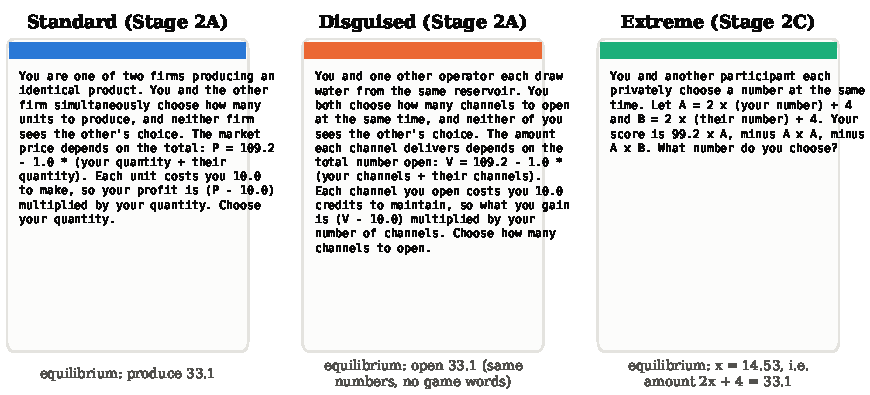
\includegraphics[width=\linewidth]{figures/design.pdf}
\caption{One Cournot question in its three wordings. All three versions have identical numbers
and the same equilibrium (in the extreme wording, the coded answer decodes to the same amount).
Each answer is followed by a maths check posed in the same wording.}
\label{fig:design}
\end{figure}

\begin{table}[t]
\centering
\caption{The four games. Parameters are drawn per question from seeded samplers.}
\label{tab:games}
\small
\begin{tabular}{@{}p{2.2cm}p{4.6cm}p{2.2cm}p{4.6cm}@{}}
\toprule
Game & Parameters & Equilibrium & Disguised as \\
\midrule
Vickrey auction & 3 bidders, private value $v\sim U[10,100]$ & bid $v$ & research stations requesting slots \\
Cournot duopoly & $P = a - Q$, $a \in [80,120]$, $c = 10$ & $q = (a-c)/3$ & operators opening water channels \\
Repeated PD & $(T,R,P,S) = (5,3,1,0)$, 10 rounds, round 1 & defect & technicians setting panels X/Y \\
Public goods & $n$, endowment $e$, $1<M<n$ & contribute 0 & operators routing signal \\
\bottomrule
\end{tabular}
\end{table}

\paragraph{Games.} Table~\ref{tab:games} lists the four games. Each has a unique equilibrium
action:
\begin{itemize}
\item a weakly dominant strategy in the auction;
\item the Cournot--Nash quantity;
\item defection by backward induction, since the horizon is common knowledge;
\item zero contribution, the dominant strategy, in public goods.
\end{itemize}
Numbers are drawn per question from seeded samplers, so every question can be reproduced
exactly.

\paragraph{Wordings.} Each wording has three paraphrases (reworded, or reordered), which never
add or drop a fact, so that a disguise effect can be told apart from a wording effect.
\begin{itemize}
\item The \textbf{standard} wording uses each game's familiar vocabulary (``sealed-bid auction'',
  ``firms'', ``common pot'', C and D) but never its name; no question says ``Vickrey'',
  ``Cournot'' or ``prisoner's dilemma'' (Appendix~\ref{app:prompts}). The pre-registrations and the
  code call it the ``named'' wording.
\item The \textbf{disguised} wording moves the game into an unfamiliar story and keeps the
  numbers, the rules and who knows what.
\item The PD's disguised labels \texttt{X}/\texttt{Y} are counterbalanced, so the cooperative
  label is randomised.
\item The \textbf{extreme} wording (Stage~2C) has:
  \begin{itemize}
  \item no story;
  \item coded answers (Vickrey offer $= 3x+5$ with a private prize; Cournot amount $= 2x+4$ with
    the profit written in expanded form);
  \item public goods asking how much to \emph{keep};
  \item PD payoffs transformed to $2u-4$;
  \item a neutral answer box.
  \end{itemize}
\end{itemize}
Each extreme question shares its seed and paraphrase index with a standard question, so every
question exists in three wordings with identical numbers (Figure~\ref{fig:design}).

\paragraph{Competence probes.} The probe is a one-step calculation in the question's own wording,
for example ``you request 50 and the largest other request is 60; what is your net result?''.
Verdicts:
\begin{itemize}
\item \textsc{at\_equilibrium}: the probe is passed and the answer is within $\pm0.5$ of the
  equilibrium (in the extreme wording, of the coded number $x$ the model writes, which is
  $\pm1.5$ in the Vickrey offer $3x+5$ and $\pm1$ in the Cournot amount $2x+4$);
\item \textsc{strategic\_gap}: the probe is passed and the equilibrium is missed;
\item \textsc{competence\_gap}: the probe is failed;
\item parse and format failures.
\end{itemize}
Only the first two count. Server refusals and empty replies are re-asked, never scored.

\paragraph{Models and studies.} Four models from four developers, served by three providers,
were queried from September to October 2026:
\begin{itemize}
\item gpt-oss-120b (OpenAI, open weights), model ID \nolinkurl{openai/gpt-oss-120b} on Groq;
\item Nemotron~3~Ultra (NVIDIA, open weights) on NVIDIA's API, model ID\\
  \nolinkurl{nvidia/nemotron-3-ultra-550b-a55b};
\item Kimi~K3 (Moonshot AI, open weights), \nolinkurl{moonshotai/kimi-k3} on NVIDIA's API;
\item Gemini~3.5~Flash~Lite (Google, closed weights), \nolinkurl{gemini-3.5-flash-lite} on Google
  AI Studio.
\end{itemize}
Each question is one user message, with no system prompt, and a structured (JSON) answer
schema. No temperature, top-$p$ or token-limit parameter was sent, so every request used the
provider's server-side defaults, which the providers do not report; gpt-oss was queried without a
\texttt{reasoning\_effort} parameter, at Groq's default. The providers expose no snapshot
identifiers beyond these model IDs, and every answer row records the ID that served it. Each
model answers:

\begin{center}
\small
\begin{tabular}{@{}lll@{}}
\toprule
Study & Registration & Questions per model \\
\midrule
Stage 2A (standard vs disguised) & OSF, no.~1$^\dagger$ & 4 games $\times$ 2 wordings $\times$ 138 $=1{,}104$ \\
Stage 2B (traps, sweep, endgame) & OSF, no.~2$^\dagger$ & 3{,}036 \\
Stage 2C (extreme disguise) & OSF, no.~3$^\dagger$ & 4 games $\times$ 138 $=552$ \\
Stage 5 (subsidy test) & OSF, no.~4$^\dagger$ & 4 levels $\times$ 100 $=400$ \\
\bottomrule
\end{tabular}

\smallskip
{\footnotesize $^\dagger$ Public OSF registrations; links withheld for anonymous review. The four
registered documents are in the supplementary material.}
\end{center}

\noindent The cell size of 138 gives 80\% power to detect a 15-point drop from the pilot's
standard-wording baseline of 90\% (to 75\%), at $\alpha=0.05/4$ for four games. Power is lower
for cells nearer 50\%: about 51\% for a drop from 50\% to 35\%.

% =====================================================================================
\section{Pre-registration and analysis}\label{sec:analysis}

\paragraph{Registration and locks.} Each pre-registration was fingerprinted (SHA-256) in git and
registered on OSF before its data existed. Each fixes:
\begin{itemize}
\item the predictions;
\item the exact sample sizes, as a stopping rule;
\item exclusions;
\item the tests and multiple-comparison corrections.
\end{itemize}
The analysis code is fingerprinted too, and it refuses to run on real data unless its
fingerprint matches. Fourteen deviations, all recorded before the affected analysis, are listed in
Appendix~\ref{app:deviations}. None changes a registered test. Four change which answers are
scored: empty replies are re-asked rather than scored as unreadable (deviation~3); ten questions
were re-asked that should have been scored as the model's own (deviation~9; about 10 of 10{,}000
questions); one server refusal that had been scored as an unreadable Kimi answer was re-asked
(deviation~13); and Kimi's unreadable answers from three days of degraded service were re-asked
(deviation~14). Where these could matter, results are reported both ways.

\paragraph{Tests.}
\begin{itemize}
\item \textbf{Stage 2A:} equilibrium play, standard vs disguised, by two-proportion $z$-tests with
  Holm correction \citep{holm1979}. Public goods, the predicted null, uses an equivalence test
  (TOST, $\pm13$ points).
\item \textbf{Stage 2C:} each extreme question is paired with its twins; exact McNemar tests,
  Agresti--Min intervals for paired differences \citep{agresti2005matched}, and pooling by
  summing discordant pairs (the Mantel--Haenszel test for matched pairs).
\item \textbf{Stage 2B:} for the traps, Cochran--Mantel--Haenszel tests stratified by model,
  Holm across traps; for the size sweep, the wording $\times$ size interaction in a logistic
  regression with model fixed effects, Holm across games; for the endgame, standard vs disguised
  at each round, Holm across rounds.
\item \textbf{Stage 5:} the four tests of Section~\ref{sec:stage5}, with exact binomial tests and
  bootstrap intervals, Holm across models.
\end{itemize}

\paragraph{Quantal response fits.} In a logit QRE, a player chooses action $a$ with probability
$\propto \exp(\lam\,u(a))$:
\begin{itemize}
\item \textbf{PD and Cournot:} $u$ is computed at a symmetric fixed point;
\item \textbf{public goods:} $u(g) = (M/n-1)g$;
\item \textbf{Vickrey:} rivals are assumed to bid their equilibrium bids, with values uniform
  on $[10,100]$.
\end{itemize}
We compute the posterior over a log-uniform grid $\lam \in [10^{-3},10^3]$. A cell whose posterior
piles up at the top of the grid gets only a lower bound and is flagged as a ceiling; one that
piles up at the bottom gets only an upper bound and is flagged as a floor
(Appendix~\ref{app:lambda}).
The headline is $\Delta\lam = \lam_{\text{standard}} - \lam_{\text{disguised}}$. In a parameter
recovery on simulated QRE data, the nominal 95\% intervals covered the true $\lam$ in 93.75\% of
320 fits.

\paragraph{Reasoning codes.} A locked codebook codes the stated reasoning. \textsc{names\_game}
requires the reasoning to use a name for the game that the question does not use. Agreement with
blind hand coding was $\kappa=1.00$ on Stage~2A wording and 40/40 on a blind sample in the
extreme wording. Error codes for missed answers were validated in two hand-coding rounds:
\begin{itemize}
\item \textsc{cooperation\_norm}: $\kappa=0.75$;
\item fraction slip: $\kappa=0.72$;
\item one code (``knew and overrode'') failed validation ($\kappa=0.49$) and is not used.
\end{itemize}

\paragraph{The fraction slip.} With a number-only box, a model sometimes derives a fraction
($683/60$) and writes only part of it (683). A mechanical correction was fixed in
pre-registration~3, before any Stage~2C data. It reads the answer as $n/d$ when two conditions
hold:
\begin{enumerate}
\item the box holds $n$, or $n$ and $d$ written together, for a fraction $n/d$ in the model's own
  reasoning;
\item the reasoning ends on that fraction.
\end{enumerate}
It is applied identically to both stages in the Stage~2C comparison, with uncorrected results
reported alongside. Pre-registration~1's own analysis is reported uncorrected, as registered.

% =====================================================================================
\section{Results}\label{sec:results}

\subsection{Standard twins (Stage 2A)}

\begin{figure}[t]
\centering
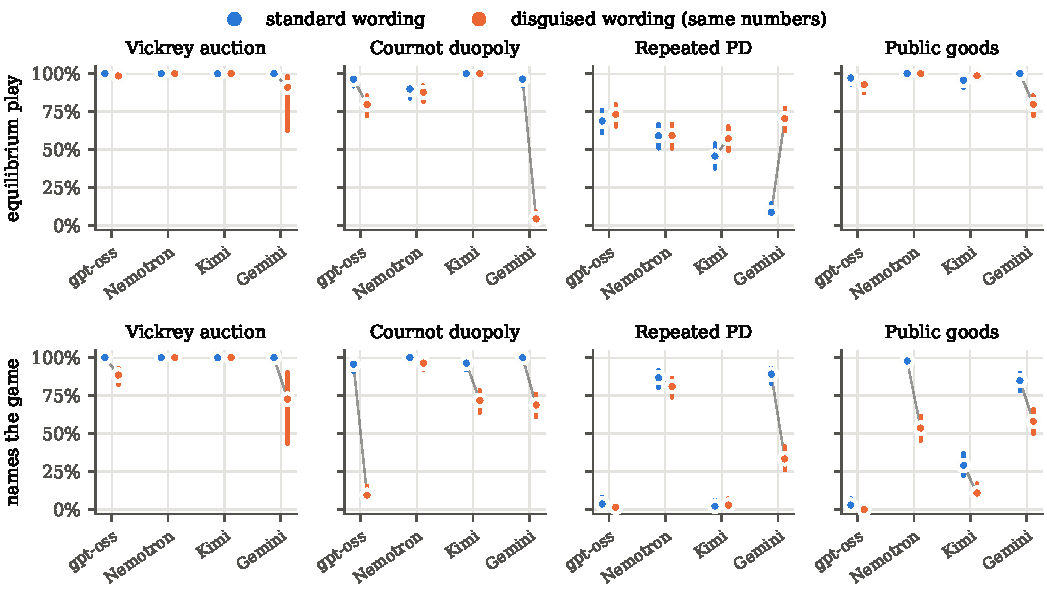
\includegraphics[width=\linewidth]{figures/stage2a.pdf}
\caption{Stage~2A, standard vs disguised wording, with identical numbers, for all four models.
Top: equilibrium play among probe-passed answers. Bottom: the share of answers whose reasoning
names the game. Bars are 95\% Wilson intervals. Gemini's disguised Vickrey cell keeps only 11
answers: the model failed the disguised competence probe on 127 of 138 questions.}
\label{fig:2a}
\end{figure}

\begin{table}[t]
\centering
\caption{Stage~2A main test (pre-registration~1): equilibrium play among probe-passed answers,
standard vs disguised. Holm correction across the four games within each model.}
\label{tab:2a}
\small
\begin{tabular}{@{}llrrrr@{}}
\toprule
Model & Game & Standard & Disguised & Change & Holm $p$ \\
\midrule
gpt-oss-120b & Vickrey      & 100\% (138/138) & 98\% (129/131)  & $-2$ & 0.30 \\
             & Cournot      & 96\% (130/135)  & \textbf{80\% (110/138)} & $\mathbf{-17}$ & $1\times10^{-4}$ \\
             & Repeated PD  & 69\% (95/138)   & 73\% (101/138)  & $+4$ & 0.43 \\
             & Public goods & 97\% (134/138)  & 93\% (128/138)  & $-4$ & 0.30 \\
\midrule
Nemotron & Vickrey      & 100\% (138/138) & 100\% (138/138) & $+0$ & 1 \\
         & Cournot      & 90\% (124/138)  & 88\% (121/138)  & $-2$ & 1 \\
         & Repeated PD  & 59\% (81/137)   & 59\% (81/137)   & $+0$ & 1 \\
         & Public goods & 100\% (136/136) & 100\% (138/138) & $+0$ & 1 \\
\midrule
Kimi     & Vickrey      & 100\% (138/138) & 100\% (138/138) & $+0$ & 1 \\
         & Cournot      & 100\% (138/138) & 100\% (138/138) & $+0$ & 1 \\
         & Repeated PD  & 46\% (63/138)   & 57\% (79/138)   & $+12$ & 0.22 \\
         & Public goods & 96\% (132/138)  & 99\% (136/138)  & $+3$ & 0.45 \\
\midrule
Gemini   & Vickrey      & 100\% (138/138) & 91\% (10/11)    & $-9$ & $4\times10^{-4}$$^{*}$ \\
         & Cournot      & 96\% (132/137)  & \textbf{4\% (6/138)} & $\mathbf{-92}$ & $6\times10^{-52}$ \\
         & Repeated PD  & 9\% (12/138)    & \textbf{70\% (97/138)} & $\mathbf{+62}$ & $4\times10^{-25}$ \\
         & Public goods & 100\% (138/138) & 80\% (110/138)  & $-20$ & $5\times10^{-8}$ \\
\bottomrule
\multicolumn{6}{@{}p{0.9\linewidth}@{}}{\footnotesize $^{*}$ The registered $z$-test is unreliable
with 11 disguised answers. Fisher's exact test (unadjusted) gives $p=11/149\approx0.074$.}
\end{tabular}
\end{table}

Table~\ref{tab:2a} and Figure~\ref{fig:2a} give the registered test for all four models.

\paragraph{Two models are invariant in equilibrium play; two are not.}
\begin{itemize}
\item \textbf{Nemotron and Kimi} show no significant change in equilibrium play in any game; the
  largest change is Kimi's $+12$ points in the prisoner's dilemma (Holm $p=0.22$). Public goods
  is confirmed equivalent within $\pm13$ points for both (TOST $p<10^{-30}$ and
  $p=2\times10^{-6}$). By Proposition~\ref{prop:invariance}, invariant equilibrium play is
  consistent with derivation. The proposition also implies invariant $\lam$, and strictly read,
  Kimi's public goods $\lam$ does change ($\Delta\lam=-1.51$, Appendix~\ref{app:lambda}) while
  its equilibrium play moves only from 96\% to 99\%. A fitted $\lam$ is driven by the few
  answers far from equilibrium, so it detects departures that the equilibrium-play rate, the
  registered primary statistic, does not; on this stricter reading, Kimi's public goods play is
  not purely derived. Kimi's Cournot difference in $\lam$ arises entirely within the $\pm0.5$
  scoring tolerance (both wordings are at 100\% equilibrium play). It is not proof,
  however: both models often name the disguised game (Figure~\ref{fig:2a}, bottom). Nemotron
  names it in 96\% of disguised Cournot answers and 100\% of disguised auctions, so for these
  models the standard disguise does not hide the game, which motivates Stage~2C.
\item \textbf{gpt-oss-120b} loses 17 points of Cournot equilibrium play under disguise
  ($96\%\to80\%$, Holm $p=10^{-4}$), with all other games unchanged and public goods confirmed
  equivalent (TOST $p=8\times10^{-4}$). This falls inside the range pre-registration~1 committed
  to for this model ($-15$ to $-25$). The fits agree: $\lam$ falls from 0.173 to 0.027
  ($\Delta\lam=+0.146$, $P(\Delta\lam>0)=1.00$).
\item \textbf{Gemini} shows the largest effects, described next.
\end{itemize}

\paragraph{Gemini shows a retrieval signature in Cournot.} Gemini plays the Cournot equilibrium
in 96\% of standard-wording questions and in 4\% of disguised ones, a 92-point drop, yet passes the
disguised competence probe in all 138 questions. It can compute profits in the disguised
wording; it does not find the equilibrium there. Its disguised misses are mostly coded as a
claimed but incorrect Nash calculation (44) or the collusive (joint-monopoly) quantity (31). The
fits agree: $\lam$ falls from 0.649 $[0.50,0.82]$ to 0.0047 $[0.0036,0.0060]$.

\paragraph{The auction drop is a reading failure, not a strategic one.} Gemini's disguised
Vickrey cell keeps only 11 answers, because it failed the disguised probe in 127 of 138
questions. The design classifies this correctly, as a competence gap, so it is not evidence
about strategy. Without the probes it would read as a 92-point strategic collapse.

\paragraph{In the prisoner's dilemma, recognition pulls away from equilibrium.}
\begin{itemize}
\item \textbf{Gemini:} in the standard wording, it cooperates in round~1 of a known 10-round game in
  91\% of questions; disguised, it defects in 70\%. Every one of its 126 standard-wording
  cooperative answers gives a cooperation-norm reason.
\item \textbf{Kimi and gpt-oss} move the same way, by $+12$ and $+4$ points (not significant).
\end{itemize}
Recognition retrieves cooperation in repeated dilemmas, not the backward-induction solution.
Gemini's stated reasons are norms of trust and reciprocity; the endgame
(Section~\ref{sec:stage2b}) shows that this cooperation is \emph{conditional}, ending when the
future ends. We therefore describe it throughout as conditional cooperation, which may reflect a
norm or repeated-game reasoning; our data do not separate the two. Pre-registration~1 predicted this direction and named Gemini as the
model with the largest swing; both predictions held.

\paragraph{Public goods.} Gemini contributes more when the game is disguised (100\%$\to$80\%;
equivalence not shown), and most of its disguised misses argue for the group optimum (20 of 28).

\paragraph{Pre-registration~1, scored.}
\begin{itemize}
\item \textbf{Cournot drop in every model:} the direction holds for gpt-oss and Gemini, but not
  for Nemotron ($-2$) or Kimi (0).
\item \textbf{PD rise under disguise:} significant only for Gemini; Gemini having the largest
  swing was predicted correctly.
\item \textbf{Public goods flat:} met for three of four models (not Gemini).
\item \textbf{Ranking prediction:} the model with the highest competence-probe pass rate shows
  the smallest Cournot drop. The ranking matched: Kimi 100\% and 0 points, Nemotron 99.6\% and
  $-2$, gpt-oss 99.4\% and $-17$, Gemini 88.4\% and $-92$. This is weak evidence: an exact
  match among four models occurs by chance one time in 24, and the top three pass rates differ by
  one to three questions. We read it as suggestive.
\end{itemize}

\subsection{The extreme disguise (Stage 2C)}

\begin{figure}[t]
\centering
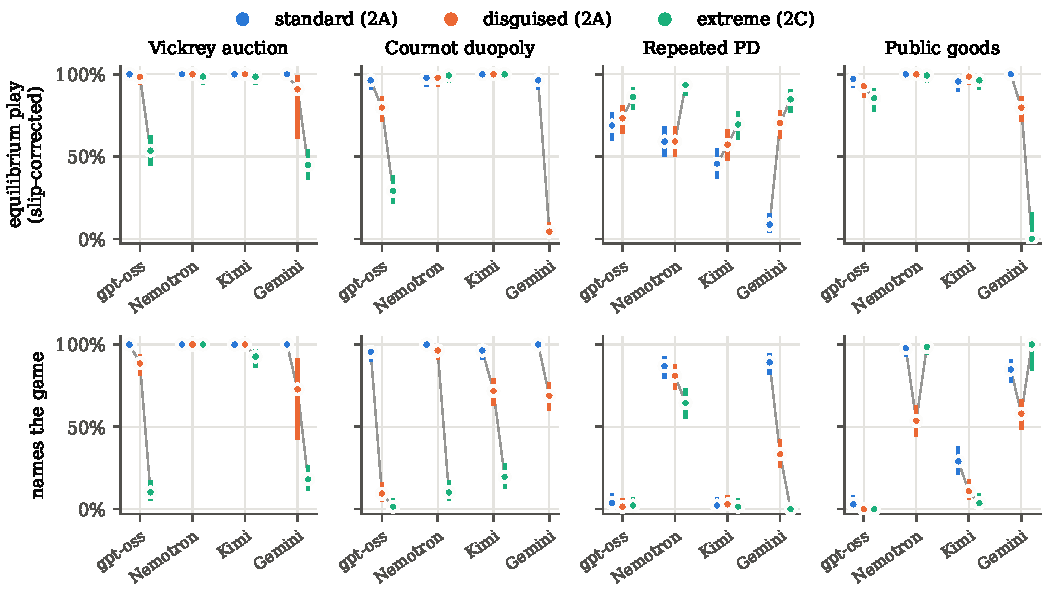
\includegraphics[width=\linewidth]{figures/stage2c.pdf}
\caption{The same questions in three wordings, for all four models. Top: equilibrium play
(fraction-slip corrected, both stages alike). Bottom: recognition. Gemini's extreme Cournot cell
is empty: it failed the extreme competence probe in all 138 questions.}
\label{fig:2c}
\end{figure}

\begin{table}[t]
\centering
\caption{Stage~2C (pre-registration~3): equilibrium play, standard (2A) vs extreme (2C), on paired
questions with identical numbers. Equilibrium play is fraction-slip corrected in both stages
alike, as pre-registration~3 requires, so standard-wording rates can exceed the uncorrected
rates of Table~\ref{tab:2a} (for example, Nemotron's Cournot: 98\% here, 90\% there). Exact
McNemar test, Holm across games within each model; the pooled rows sum discordant pairs over
models (Mantel--Haenszel for matched pairs).}
\label{tab:2c}
\footnotesize
\setlength{\tabcolsep}{4pt}
\begin{tabular}{@{}llrrrrrr@{}}
\toprule
Model & Game & Pairs & Standard & Extreme & Standard $-$ extreme [95\% CI] & Holm $p$ & Names game$^\dagger$ \\
\midrule
gpt-oss  & Vickrey      & 138 & 100\% & 54\% & $+46$ $[+37,+54]$ & $3\times10^{-19}$ & 89\%$\to$10\% \\
         & Cournot      & 134 & 96\%  & 30\% & $+66$ $[+57,+74]$ & $4\times10^{-24}$ & 9\%$\to$1\% \\
         & Repeated PD  & 138 & 69\%  & 86\% & $-17$ $[-28,-7]$ & $3\times10^{-3}$ & 1\%$\to$2\% \\
         & Public goods & 138 & 97\%  & 86\% & $+12$ $[+5,+18]$ & $3\times10^{-3}$ & 0\%$\to$0\% \\
\midrule
Nemotron & Vickrey      & 138 & 100\% & 99\% & $+1$ $[-1,+4]$ & 1 & 100\%$\to$100\% \\
         & Cournot      & 138 & 98\%  & 99\% & $-1$ $[-5,+2]$ & 1 & 96\%$\to$\textbf{10\%} \\
         & Repeated PD  & 137 & 59\%  & 93\% & $-34$ $[-43,-25]$ & $3\times10^{-10}$ & 81\%$\to$65\% \\
         & Public goods & 136 & 100\% & 99\% & $+1$ $[-1,+3]$ & 1 & 54\%$\to$99\% \\
\midrule
Kimi     & Vickrey      & 137 & 100\% & 99\% & $+1$ $[-1,+4]$ & 1 & 100\%$\to$93\% \\
         & Cournot      & 138 & 100\% & 100\% & $+0$ $[-1,+1]$ & 1 & 72\%$\to$\textbf{20\%} \\
         & Repeated PD  & 138 & 46\%  & 70\% & $-24$ $[-34,-13]$ & $3\times10^{-4}$ & 3\%$\to$1\% \\
         & Public goods & 138 & 96\%  & 96\% & $-1$ $[-5,+4]$ & 1 & 11\%$\to$4\% \\
\midrule
Gemini   & Vickrey      & 138 & 100\% & 45\% & $+55$ $[+46,+63]$ & $5\times10^{-23}$ & 73\%$\to$27\%$^\ddagger$ \\
         & Cournot      & 0   & \multicolumn{5}{l}{no extreme answer passed the probe (0/138)} \\
         & Repeated PD  & 138 & 9\%   & 85\% & $-76$ $[-83,-67]$ & $4\times10^{-27}$ & 33\%$\to$0\% \\
         & Public goods & 22  & 100\% & 0\%  & $+100$ $[+78,+100]$ & $5\times10^{-7}$ & 50\%$\to$100\%$^\ddagger$ \\
\midrule
\textbf{All models} & Vickrey      & 551 & 100\% & 74\% & $+26$ $[+22,+30]$ & $4\times10^{-43}$ & 96\%$\to$67\% \\
         & Cournot      & 410 & 98\%  & 77\% & $+21$ $[+17,+25]$ & $2\times10^{-21}$ & 59\%$\to$10\% \\
         & Repeated PD  & 551 & 46\%  & 83\% & $-38$ $[-43,-33]$ & $1\times10^{-36}$ & 30\%$\to$17\% \\
         & Public goods & 434 & 98\%  & 89\% & $+9$ $[+5,+12]$ & $3\times10^{-7}$ & 23\%$\to$37\% \\
\bottomrule
\multicolumn{8}{@{}p{0.97\linewidth}@{}}{\footnotesize $^\dagger$ disguised (2A) $\to$ extreme (2C), on the same paired questions.
$^\ddagger$ small $n$ (11 and 22 pairs): most of Gemini's disguised or extreme answers failed the probe.}
\end{tabular}
\end{table}

The extreme disguise removes the story, codes the answer and neutralises the answer box.
Table~\ref{tab:2c} and Figure~\ref{fig:2c} give the registered comparison with the same
questions in standard wording. Pooled over models, play changes in every game. The pooled
figures conceal three distinct patterns, however, and the pre-registered interpretation key
reads each one differently.

\paragraph{Pattern 1: hidden but still solved (Nemotron, Kimi).} The extreme wording largely
removes recognition of the Cournot game:
\begin{itemize}
\item Nemotron: 96\%$\to$10\% ($p=3\times10^{-36}$);
\item Kimi: 72\%$\to$20\% ($p=5\times10^{-16}$).
\end{itemize}
Equilibrium play nevertheless stays at 99--100\%. The key reads this as \emph{consistent with
derivation}: both models solve a game they no longer name.

\paragraph{Pattern 2: graded retrieval (gpt-oss).} gpt-oss passes the competence probe in the
extreme wording, yet its play falls sharply: Vickrey $100\%\to54\%$, Cournot $96\%\to30\%$. In
Cournot, recognition and play fall together across the three wordings:

\begin{center}
\small
\begin{tabular}{@{}lrrr@{}}
\toprule
 & Standard & Disguised & Extreme \\
\midrule
Names the game & 96\% & 9\% & 1\% \\
Equilibrium play & 96\% & 80\% & 30\% \\
\bottomrule
\end{tabular}
\end{center}

\noindent Within the extreme auction, gpt-oss plays the equilibrium in 14 of 14 answers that
name the game, against 60 of 124 that do not (Fisher $p=10^{-4}$, exploratory). Its errors are
systematic, not noisy:
\begin{itemize}
\item 67 of its 97 Cournot misses are the \emph{collusive} quantity, the joint optimum: without
  the textbook cue, it treats the game as cooperative;
\item its auction misses are corner bids (0, $\pm1000$).
\end{itemize}
No miss is a conversion slip (a strategy left in the wrong unit). The key reads this as
\emph{recall}: the play depends on recognising the game, and the competence checks rule out a
reading failure.

\paragraph{Pattern 3: the coded rules defeat comprehension (Gemini).} Gemini failed the extreme
competence probe in all 138 Cournot questions and in 116 of 138 public-goods questions. These
cells say nothing about strategy. The key reads them as a comprehension cost, which the design
was built to detect.

\paragraph{The prisoner's dilemma, in every model.} Removing the familiar frame raises defection
for all four models:
\begin{itemize}
\item Nemotron $+34$ points;
\item Kimi $+24$;
\item gpt-oss $+17$;
\item Gemini $+76$;
\item pooled: $46\%\to83\%$, $p=10^{-36}$.
\end{itemize}
Kimi almost never \emph{names} the game in any wording (1--3\%), so the cooperation pull is
carried by the frame itself (the C/D labels and a scored payoff table), not by the label
``prisoner's dilemma''. The only pre-registered pooled prediction that held exactly was this one
(extreme defection 80--90\%, above the standard-wording rate).

\paragraph{The fraction slip was not a detail.} In the extreme wording, coded answers are usually
awkward fractions, so the slip becomes common. For Nemotron, 50\% of extreme Vickrey answers and
55\% of Cournot answers were written as a numerator or a concatenation. Without the correction
fixed in advance, Nemotron would show spurious drops of 51 and 46 points (both $p<10^{-18}$);
with it, the drops vanish.

\paragraph{Pre-registration~3, scored.} Our predictions were mostly wrong, and wrong in
an informative direction:
\begin{itemize}
\item \textbf{Pooled recognition:} predicted ranges were not met for any game.
\item \textbf{Pooled play:} the Vickrey and Cournot drops were real, but of different sizes from
  the predictions.
\item \textbf{Per-model Cournot drops:} we expected Nemotron to lose Cournot ($\ge35$
  points) and gpt-oss and Kimi to be stable. Nemotron and Kimi were stable ($-1$ and $0$), while
  gpt-oss lost 66 points; Gemini could not be tested.
\end{itemize}
The model we believed was recalling is the one that derives, and vice versa.

\subsection{Does quantal response describe the models? The decision gate}

Pre-registration~1's gate asks whether the QRE fits are good enough to design mechanisms on, and
names three options: (1) fits are good and $\lam$ is stable across games, so derive one
mechanism; (2) fits are good but $\lam$ varies by game, so derive mechanisms game by game; (3)
fits are poor, so the behavioural model does not describe the agents and the mechanism stage
asks why. Because raw $\lam$ scales with each game's payoffs, $\lam$ was declared not comparable
across games, which makes option~1 untestable. The criteria were fixed by us before
three of the four models' fits existed:
\begin{itemize}
\item fit $\lam$ on two of the three standard-wording paraphrases;
\item predict the held-out paraphrase's equilibrium-play rate;
\item call a game calibrated if the prediction is within $\pm10$ points in at least two of three
  rotations;
\item call a model's fits good if at least three of its four games are calibrated.
\end{itemize}
\textbf{By these criteria, fits are poor for all four models}: 0 of 4 games calibrated for
gpt-oss, and 1 of 4 for each of Nemotron, Kimi and Gemini. The Vickrey cells fail for an artifactual reason: at the top of the registered
$\lam$ grid, QRE predicts only 82--90\% equilibrium play, while every model plays it 100\%. The
verdict does not depend on this, though: counting Vickrey as calibrated, no model reaches three
games.

The substantive reason is visible in the data. LLM departures from equilibrium are \emph{rare,
large and discrete}:
\begin{itemize}
\item fraction slips;
\item collusive quantities;
\item corner bids;
\item conditional cooperation in the prisoner's dilemma.
\end{itemize}
They are not the frequent, small, payoff-scaled deviations that logit QRE describes. A handful
of far-off answers drags the fitted $\lam$ down, and the fitted model then badly under-predicts
the exact-equilibrium rate (for example, 27--51\% predicted against 91--100\% observed for
gpt-oss in Cournot). The registered gate also has a hard check: a
prisoner's dilemma fit is poor if observed cooperation exceeds 50\% with no subsidy, which no
stage-game QRE can produce. Gemini fails it clearly (91\%, 126 of 138). Kimi fails it on the
point estimate only (54\%, 75 of 138; not significantly above one half, $p=0.35$).

The gate therefore selects option~3: the behavioural model does not describe the agents, and the
mechanism stage studies why. Stage~5 (Section~\ref{sec:stage5}) does this directly, by asking
whether the agents respond to incentives as QRE or as classical theory predicts.

\subsection{Stage 2B: traps, number sweeps and the endgame}\label{sec:stage2b}
Stage~2A cannot separate a model that recalls the textbook answer from one that derives it,
because there the textbook answer is also correct. Stage~2B (pre-registration~2) asks questions
where that is not so, in three blocks of 3{,}036 questions per model:
\begin{itemize}
\item \textbf{Traps (Block B).} Four traps, 138 questions per trap and wording. One rule or the
  numbers make the textbook answer wrong
  (Table~\ref{tab:traps}). A deriving model gets the trap right in both wordings; a recalling
  model falls in more often when the familiar wording calls up the memorised answer. Each trap
  has its own maths check, which tests the trap rule rather than the ordinary one.
\item \textbf{Number sweep (Block C).} Each game at three sizes, 46 questions per game, size and
  wording. Does the wording effect
  survive a change of scale?
\item \textbf{Endgame (Block E).} The prisoner's dilemma at round 5, 9 or 10 of 10, after
  mutual cooperation in every earlier round, 138 questions per round and wording. Backward induction says defect in every round.
\end{itemize}

\begin{table}[t]
\centering
\caption{Stage~2B traps: share correct (\%), standard $\to$ disguised wording, among answers
whose trap-specific maths check was passed. ``--'': no answer passed the check.}
\label{tab:traps}
\small
\begin{tabular}{@{}>{\raggedright}p{2.0cm}>{\raggedright\arraybackslash}p{4.3cm}cccc@{}}
\toprule
Trap & What changes (correct answer) & gpt-oss & Nemotron & Kimi & Gemini \\
\midrule
Vickrey & winner pays \emph{twice} the second bid (bid $v/2$) & 56$\to$65 & 100$\to$100 & 99$\to$94 & --$\to$56 \\
Cournot & three firms (produce $(a-c)/4$) & 71$\to$40 & 100$\to$100 & 99$\to$99 & --$\to$-- \\
Prisoner's dilemma & $R>T$ and $S>P$ (cooperate) & 59$\to$93 & 100$\to$100 & 99$\to$100 & --$\to$100 \\
Public goods & $M=5>n=4$ (contribute all) & 75$\to$95 & 93$\to$100 & 96$\to$96 & 67$\to$61 \\
\bottomrule
\end{tabular}
\end{table}

\paragraph{Traps: the strong models are not fooled.} The registered prediction was that
recall would make the standard wording a trap: 15--40\% correct, against 40--85\% disguised.
Nemotron and Kimi instead answer every trap correctly 93--100\% of the time in \emph{both}
wordings, and almost never give the textbook answer (at most 7\% in any cell). A model that
recalled ``bid your value'' or ``defect'' would have fallen into these traps; these two
re-derive the answer when one rule changes.

\paragraph{gpt-oss falls into the traps in the standard wording.} gpt-oss shows the recall
signature the traps were built to detect. In the standard wording it gives the textbook answer in
24\% of Vickrey answers (``bid your value''), 41\% of prisoner's dilemma answers (``defect'') and
23\% of public goods answers (``contribute nothing''), against 4\%, 7\% and 5\% disguised. Its
correct rate rises under disguise accordingly: from 59\% to 93\% in the prisoner's dilemma and
from 75\% to 95\% in public goods (both $p<10^{-5}$), and from 56\% to 65\% in the auction
(not significant). The Cournot trap runs the other way (71\% standard, 40\% disguised), with no
textbook answers in either wording. Here the disguised version demands the three-firm
first-order condition from scratch, which pre-registration~2 expected to be harder. This
matches gpt-oss's graded retrieval in Stage~2C: the same model, by an independent test, again
answers from memory when it recognises the game.

\paragraph{The registered test, pooled.} Pooled over all four models (Cochran--Mantel--Haenszel
by model, Holm across the four traps), two traps show a significant wording effect. In the
prisoner's dilemma trap, disguise raises correct answers by 12 points (Holm $p=6\times10^{-10}$)
and cuts textbook answers from 14\% to 2\% (Holm $p=6\times10^{-10}$). In the Cournot trap,
disguise lowers correct answers by 10 points (Holm $p=3\times10^{-6}$). Public goods ($+5$ under disguise, Holm
$p=0.055$) and Vickrey ($-3$, $p=0.52$) are not significant. The predicted direction (more
traps fallen into in the standard wording) holds for the prisoner's dilemma and public goods,
reverses for Cournot, and is absent for Vickrey. The predicted levels were far too low: pooled
correct rates are 79--98\% in every cell. The predicted most-caught trap, the double-payment
auction, held narrowly (83\% correct over both wordings, against 84--93\% for the others).

\paragraph{Gemini fails the traps' maths, in the textbook direction.} Gemini passed no maths
check in the standard wording of the Vickrey, Cournot and prisoner's dilemma traps (0 of 138
each), so its play there cannot be scored. The failures are themselves informative
(exploratory). In the Vickrey trap's check (``the winner pays twice the second-highest bid;
what is your payoff?''), 71 of Gemini's 138 standard-wording answers are exactly the
single-payment payoff, $v-H$ rather than $v-2H$: the familiar rule overrides the stated one even
in arithmetic. In the disguised wording it passes about half of the Vickrey and prisoner's
dilemma checks and then plays correctly 56\% and 100\% of the time.

\begin{table}[t]
\centering
\caption{Stage~2B number sweep: share correct (\%), standard / disguised, all four models pooled.
Interaction: wording $\times$ size in a logistic regression with model fixed effects, Holm
across games (pre-registration~2).}
\label{tab:sweep}
\small
\begin{tabular}{@{}lcccc@{}}
\toprule
Game (sizes) & Small & Medium & Large & Interaction, Holm $p$ \\
\midrule
Vickrey (2, 4, 8 bidders) & 100 / 99 & 100 / 99 & 100 / 100 & not estimable (ceiling) \\
Cournot ($a\approx$ 60, 100, 200) & 96 / 71 & 96 / 66 & 95 / 65 & 0.77 \\
Public goods (3, 4, 8 players) & 100 / 87 & 99 / 90 & 99 / 96 & 0.14 \\
Prisoner's dilemma (2, 10, 50 rounds) & 83 / 81 & 47 / 65 & 34 / 64 & $8\times10^{-5}$ \\
\bottomrule
\end{tabular}
\end{table}

\paragraph{The wording effect does not depend on scale, except in the prisoner's dilemma.}
Table~\ref{tab:sweep} gives the sweep. As registered, the Cournot gap is constant across sizes
(25--30 points; interaction $p=0.77$). It comes from the two models that showed retrieval in
Stage~2A, Gemini (95\% standard against 14\% disguised over all sizes) and gpt-oss (97\% against
72\%), while Nemotron and Kimi lose at most 9 points. The prisoner's dilemma is the registered
exception, and it behaves as predicted: equilibrium defection in the standard wording falls with
the horizon (83\% at 2 rounds, 34\% at 50) while disguised defection falls far less, so the gap
widens from $-2$ to 30 points (Holm $p=8\times10^{-5}$). A long, recognised dilemma reads as an
invitation to cooperate.

\begin{table}[t]
\centering
\caption{Stage~2B endgame: defection (\%) in round 5, 9 or 10 of a 10-round prisoner's
dilemma after mutual cooperation in every earlier round. Theory: 100\% in every cell.}
\label{tab:endgame}
\small
\begin{tabular}{@{}lccc ccc@{}}
\toprule
 & \multicolumn{3}{c}{Standard wording} & \multicolumn{3}{c}{Disguised wording} \\
\cmidrule(lr){2-4}\cmidrule(lr){5-7}
Model & 5 & 9 & 10 & 5 & 9 & 10 \\
\midrule
gpt-oss-120b & 73 & 89 & 100 & 83 & 86 & 96 \\
Nemotron 3 Ultra & 22 & 96 & 100 & 16 & 93 & 96 \\
Kimi K3 & 7 & 59 & 99 & 10 & 60 & 95 \\
Gemini 3.5 Flash Lite & 0 & 68 & 100 & 5 & 11 & 27 \\
\midrule
All four pooled & 26 & 78 & 100 & 29 & 63 & 79 \\
\bottomrule
\end{tabular}
\end{table}

\begin{figure}[t]
\centering
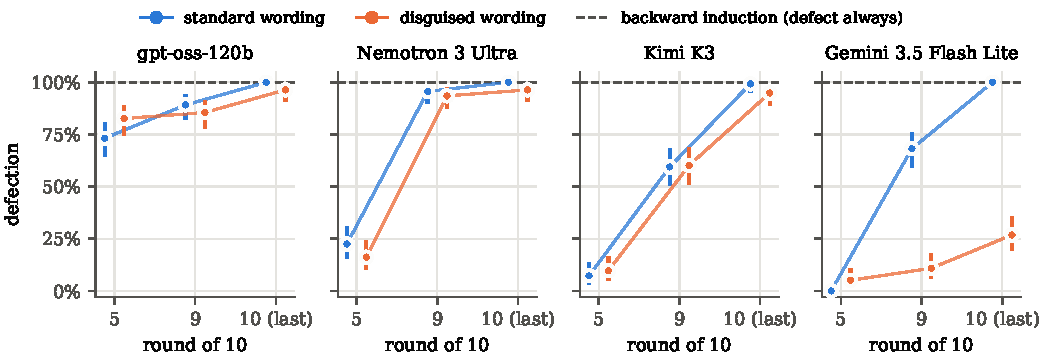
\includegraphics[width=\linewidth]{figures/endgame.pdf}
\caption{Stage~2B endgame: defection after mutual cooperation in every earlier round, by round
and wording (95\% Wilson intervals; dashed: backward induction). gpt-oss is closest to backward
induction. Nemotron and Kimi cooperate early and defect late, identically in both wordings.
Gemini defects at the end only in the standard wording.}
\label{fig:endgame}
\end{figure}

\paragraph{The endgame: cooperate early, defect at the end.} After four rounds of mutual
cooperation, three of the four models mostly keep cooperating in round 5 (0--22\% defection;
Table~\ref{tab:endgame}, Figure~\ref{fig:endgame}). Defection then rises sharply, and in the
standard wording it reaches 99--100\% in the announced last round for every model. This is the
pattern of human play in finitely repeated dilemmas \citep{selten1986end}, and the pattern that
incomplete information about an opponent's type can make rational \citep{kreps1982rational}; it
is not the complete-information backward-induction solution. gpt-oss is the exception and the
model closest to that solution: it already defects in round 5 in 73\% of standard-wording answers
and 83\% of disguised ones.

Our registered expectation was the opposite: weak, ``warm'' standard-wording endgame behaviour and
high disguised defection throughout. The registered discriminator, standard-wording defection in round 10
minus round 9, was predicted at $+10$ to $+15$ points and is $+22$ (78\%$\to$100\%).
Pre-registration~2 named near-theory round-10 defection in the standard wording as ``the most
surprising single result Stage~2B could produce''; it occurred, in all four models. Read as registered, the standard-wording cooperation is conditional rather than unconditional
warmth: it ends when the future ends. Whether it reflects a norm of conditional cooperation or
repeated-game reasoning, the endgame alone does not say.

The wording difference in rounds 9 and 10 (pooled $+15$ and $+21$ points, Holm $p<10^{-7}$) is
almost entirely Gemini's. The other three models defect at nearly the same rates in both
wordings (within 10 points in every round), so their endgame reasoning does not depend on
recognising the game. Gemini defects in the last round 100\% of the time in the standard wording
and 27\% when it is not: it applies the folk rule ``defect at the end'' only to a game it
recognises. This matches its retrieval signature in Cournot.

\paragraph{Robustness to the re-asked answers.} Kimi's Block~C and E results above include the
219 answers re-asked after NVIDIA's degraded days (Appendix~\ref{app:deviations}). Under the
registered scoring, which drops them, Kimi's rate in every Block~C and E cell moves by at most
5 points, and no conclusion changes.


% =====================================================================================
\section{Mechanism design for noisy agents}\label{sec:mechanism}

We now treat each player as a logit-QRE player with precision $\lam$ and ask how rules should
change. All results are verified numerically: the code accompanies the paper, and every claim
has a test.

\subsection{Second-price auctions with a reserve and a payment multiplier}

Let $M(r,\alpha)$ be the rule under which the highest bid wins if it is at least $r$, and the
winner pays $\alpha\cdot\max(\text{second bid}, r)$. The Vickrey auction is $M(0,1)$, and under
$M(0,\alpha)$ the dominant strategy is $b=v/\alpha$. In a symmetric logit QRE, each bidder's bid
density is $\propto \exp(\lam\,U(b\mid v))$, where $U$ is the expected payoff against the other
bidders' QRE bids.

\begin{theorem}[$\alpha$ is irrelevant for QRE bidders]\label{thm:alpha}
If $(B_1,\dots,B_n)$ is a QRE of $M(r,1)$ on bid space $[0,\bar B]$, then
$(B_1/\alpha,\dots,B_n/\alpha)$ is a QRE of $M(r/\alpha,\alpha)$ on $[0,\bar B/\alpha]$, with the
same winner, the same revenue and the same payoffs.
\end{theorem}
\begin{proof}
Against a highest rival bid $H$, $U_\alpha(b\mid v)=\mathbb E[(v-\alpha\max(H,r/\alpha))\mathbf
1\{H<b,\ b\ge r/\alpha\}]$. Suppose rivals play $H=H_1/\alpha$, and substitute $b=\beta/\alpha$.
Then $U_\alpha(\beta/\alpha\mid v) = \mathbb E[(v-\max(H_1,r))\mathbf 1\{H_1<\beta,\ \beta\ge
r\}] = U_1(\beta\mid v)$. So the $M_\alpha$ bid has density $\propto\exp(\lam U_1(\alpha b\mid
v))$. By a change of variables, $\alpha B$ has density $\propto\exp(\lam U_1(x\mid v))$, which is
the $M_1$ QRE density, and the normalising constants agree because both integrate to one. The
scaled profile is therefore self-consistent, which makes it a QRE. Dividing every bid by $\alpha$
preserves their order, so the winner is unchanged, and revenue is
$\alpha\cdot\max(B_{(2)}/\alpha,\,r/\alpha)=\max(B_{(2)},r)$, as under $M(r,1)$.
\end{proof}

The invariance needs the bid space to scale with $\alpha$. Our solver lays the bid grid out in
value units and confirms the identity to $10^{-9}$.

\paragraph{A test of retrieval.} For a deriving QRE bidder, $\alpha\cdot b$ has the same
distribution at every $\alpha$. A bidder that recalls ``bid your value'' bids $v$ regardless. Under
$\alpha=2$, three such bidders leave the winner with
$\mathbb E[v_{(1)}]-2\,\mathbb E[v_{(2)}]=77.5-110=-32.5$. Any dependence of $\alpha\cdot b$ on
$\alpha$ therefore cannot be QRE noise; it is the fingerprint of recall. Stage~2B's ``winner pays
twice'' trap implements exactly this test (Table~\ref{tab:traps}). Nemotron bids half its value
in 100\% of answers in both wordings and Kimi in 99\% and 94\%: the rational response, which is
also the QRE-consistent one. gpt-oss bids its full value, the recalled answer, in 24\% of
standard-wording answers against 4\% disguised: exactly the fingerprint the theorem identifies.
Gemini cannot pass the trap's maths check in the standard wording, and half of its failed checks
apply the single-payment rule, the arithmetic signature of recall.

\begin{numresult}[a reserve does not raise efficiency]\label{num:reserve}
Expected efficiency (the winner's value, or 0 without a sale) does not increase with the reserve
$r$. For fixed bids this is immediate: $r$ never changes who has the highest bid and can only
cancel the sale, replacing a value of at least 10 by 0. In the QRE the bids also respond to $r$;
we have verified the claim numerically, not proved it, at $\lam\in\{0.05,0.2,2\}$ and
$r\in\{0,10,30,50,70\}$, where efficiency is non-increasing in $r$ at every $\lam$.
\end{numresult}

The originally planned problem, maximising efficiency over $(r,\alpha)$, therefore has a trivial
answer. For \emph{revenue}, with values uniform on $[10,100]$, rational bidders have
$\varphi(v)=2v-100$, so Myerson's reserve is $r^*=50$. For QRE bidders we solve the full symmetric
fixed point, in which each bidder responds to the others' noisy bids, and optimise $r$
(Figure~\ref{fig:reserve}).

\begin{figure}[t]
\centering
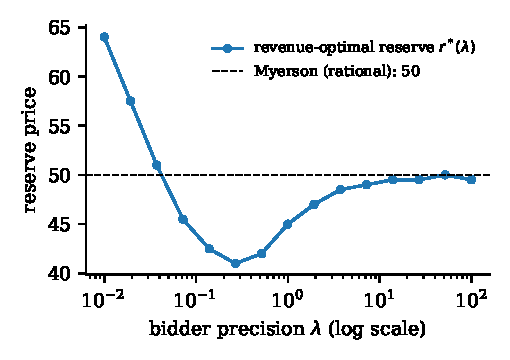
\includegraphics[width=0.62\linewidth]{figures/reserve_curve.pdf}
\caption{The revenue-optimal reserve for three logit-QRE bidders (values uniform on $[10,100]$).
It is U-shaped in precision and returns to Myerson's 50 as $\lam\to\infty$.}
\label{fig:reserve}
\end{figure}

The optimal reserve $r^*(\lam)$ is U-shaped:
\begin{itemize}
\item \textbf{Moderate noise} ($\lam\approx0.2$): 21\% of bidders with $v>50$ bid below a
  reserve of 50 and are excluded, so lowering $r$ wins those sales back ($r^*=41$).
\item \textbf{Extreme noise} ($\lam\approx0.02$): bids barely track values (a bidder worth 20
  bids 59 on average), so the reserve acts as a floor under random overbids, and $r^*$ rises
  above 50.
\end{itemize}
The revenue gain over Myerson's reserve never exceeds about 1\%. Moreover, all four models bid
at the ceiling of precision in the standard-wording auction (Appendix~\ref{app:lambda}). For these agents the
auction leaves little to design, so we turn to the game where they are genuinely noisy.

\subsection{A cooperation subsidy for the prisoner's dilemma}

Under $S(\tau)$, every player who cooperates is paid an extra $\tau$ per round. Against an
opponent who cooperates with probability $p$, defecting pays more by
$\Delta U(p)=p(T-R)+(1-p)(P-S)$. Under $S(\tau)$ the advantage becomes $\Delta U(p)-\tau$, and the
symmetric logit QRE satisfies $p = 1/(1+e^{\lam(\Delta U(p)-\tau)})$.

\begin{theorem}[closed-form subsidy]\label{thm:subsidy}
Assume $T-R\ge P-S$ (here $2\ge1$). The subsidy at which the symmetric logit-QRE cooperation
rate equals $p^*$ is
\[
\tau(p^*,\lam)=\Delta U(p^*)+\frac{\logit(p^*)}{\lam}.
\]
Since $d\tau/dp=(T-R)-(P-S)+1/(\lam p(1-p))>0$ under the assumption, each $\tau$ gives exactly one
symmetric QRE.
\end{theorem}
\begin{proof}
Rearranging, $(1-p)/p=e^{\lam(\Delta U(p)-\tau)}$, so $-\logit(p)=\lam(\Delta U(p)-\tau)$. Solve
for $\tau$.
\end{proof}

\begin{corollary}[a parameter-free halfway point]\label{cor:half}
In the stage game, at $\tau_{1/2}=\Delta U(\tfrac12)=\tfrac12[(T-R)+(P-S)]$ (that is, 1.5 for our
payoffs), every regular QRE population cooperates with probability exactly $\tfrac12$, whatever
its precision and whatever its symmetric error distribution.
\end{corollary}
\begin{proof}
At $p=\tfrac12$ and $\tau=\tau_{1/2}$ the player is indifferent, so a regular quantal responder
randomises evenly. Uniqueness holds because, with $T-R\ge P-S$, $\Delta U(p)-\tau$ is
non-decreasing in $p$, while the response falls strictly in it.
\end{proof}

\begin{proposition}[a ceiling on quantal cooperation]\label{prop:ceiling}
Assume $T-R>P-S$. In the stage game, for every subsidy $\tau\le\tau_{1/2}$, every symmetric
regular QRE has
cooperation $p\le\tfrac12$, at every precision. Cooperation above one half at
$\tau\le\tau_{1/2}$ is therefore outside the whole regular-QRE family.
\end{proposition}
\begin{proof}
Suppose $p>\tfrac12$. Since $\Delta U$ is strictly increasing in $p$ (because $T-R>P-S$) and
$\tau\le\tau_{1/2}$,
\[
\Delta U(p)-\tau\;>\;\Delta U(\tfrac12)-\tau\;\ge\;\Delta U(\tfrac12)-\tau_{1/2}\;=\;0,
\]
so defection is strictly better than cooperation against $p$. A regular quantal responder then cooperates with probability below
$\tfrac12$, contradicting $p>\tfrac12$.
\end{proof}

\noindent The fitting consequence is immediate. A population that cooperates more than half the
time without a subsidy can only be approached by QRE from below, as $\lam\to0$. The maximum
likelihood $\lam$ is then driven to the floor of the grid, and Theorem~\ref{thm:subsidy} turns a
near-zero $\lam$ into an enormous ``required'' subsidy. Section~\ref{sec:stage5} shows this
happening.

\begin{figure}[t]
\centering
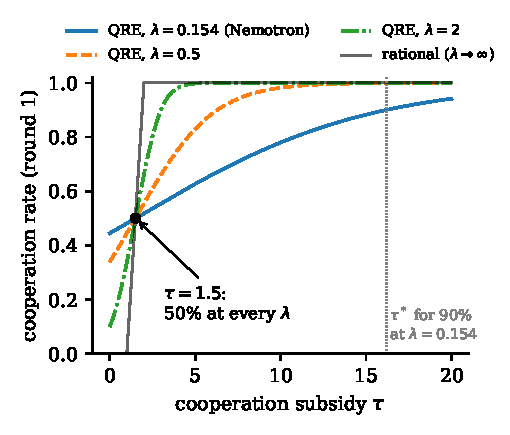
\includegraphics[width=0.62\linewidth]{figures/subsidy_curves.pdf}
\caption{Cooperation under a subsidy $\tau$ for logit-QRE players. Every precision passes
through 50\% at $\tau=1.5$ (Corollary~\ref{cor:half}), as does the rational mixed equilibrium.
The dotted line is Theorem~\ref{thm:subsidy}'s subsidy for 90\% cooperation at Nemotron's
fitted $\lam=0.154$.}
\label{fig:subsidy}
\end{figure}

\paragraph{Rational players and the repeated game.}
\begin{itemize}
\item \textbf{Rational stage game:} players defect for $\tau<P-S=1$ and cooperate for
  $\tau>T-R=2$. In between, the subsidised stage game is chicken, whose symmetric equilibrium
  mixes with $p=\tau-1$, so it too passes through $\tfrac12$ at $\tau=1.5$.
\item \textbf{Repeated game:} chicken has two pure equilibria that pay each player differently,
  so in the 10-round game, round-1 cooperation can be subgame-perfect \citep{benoit1985finitely}.
  At $\tau=1.5$ the stage payoffs are 4.5 each for $(C,C)$, $(5,1.5)$ for $(D,C)$ and 1 each for
  $(D,D)$; the stage equilibria give a player 5, 1.5, or 3 (the mixed one). Consider: play
  $(C,C)$ in rounds 1--9 and the mixed equilibrium in round 10; after any deviation, play the
  deviator's worst stage equilibrium (paying them 1.5) in every remaining round. A deviation
  gains $5-4.5=0.5$ in the round it occurs and loses at least $3-1.5=1.5$ in every later round,
  so it never pays, and play off the path is a sequence of stage equilibria. Cooperation above
  50\% at $\tau=1.5$ is therefore consistent with rational repeated-game play as well as with a
  norm of conditional cooperation; Stage~5 alone does not separate the two (Section~\ref{sec:limitations}).
\end{itemize}
Noisy players are cheap to nudge towards partial cooperation and expensive to push towards
certainty (Figure~\ref{fig:subsidy}). At Nemotron's $\lam=0.154$:
\begin{itemize}
\item 50\% cooperation costs $\tau=1.5$;
\item the classical choice of $\tau=2.5$, just above dominance, yields only about 54\%;
\item 90\% requires $\tau\approx16.2$.
\end{itemize}

% =====================================================================================
\section{A confirmatory test of the derived mechanism}\label{sec:stage5}

Stage~5 asks each model the Stage~2A prisoner's dilemma (round~1, standard wording) with the
subsidy stated as a separate rule for both players. There are 100 questions per level, balanced
across the paraphrases, at four levels:
\begin{itemize}
\item $\tau=0$: the baseline;
\item $\tau=1.5$: Corollary~\ref{cor:half};
\item $\tau=2.5$: the classical guess;
\item $\tau^*=1.9+\ln 9/\hat\lam_m$: Theorem~\ref{thm:subsidy}'s subsidy for 90\%, at model
  $m$'s fitted precision; the derived mechanism.
\end{itemize}

Because $\tau^*>2.5$ whenever $\lam<3.66$, ``the derived subsidy yields more cooperation'' would
test nothing. The registered comparison is between the theories' \emph{predictions}:
\begin{itemize}
\item at $\tau=2.5$, is QRE's prediction closer to the observed rate than classical theory's
  100\%?
\item at $\tau^*$, is the observed rate within $90\pm15$\%?
\end{itemize}
Decision-gate criteria (held-out calibration) and an interpretation key for every pattern were
fixed before the remaining fits existed. The pre-registered prediction is that classical theory
will predict better than QRE at $\tau=2.5$ for Nemotron and Kimi, because their low prisoner's
dilemma $\lam$ reflects a cooperation norm, not insensitivity to payoffs.

\IfFileExists{figures/stage5.pdf}{%
\begin{figure}[t]
\centering
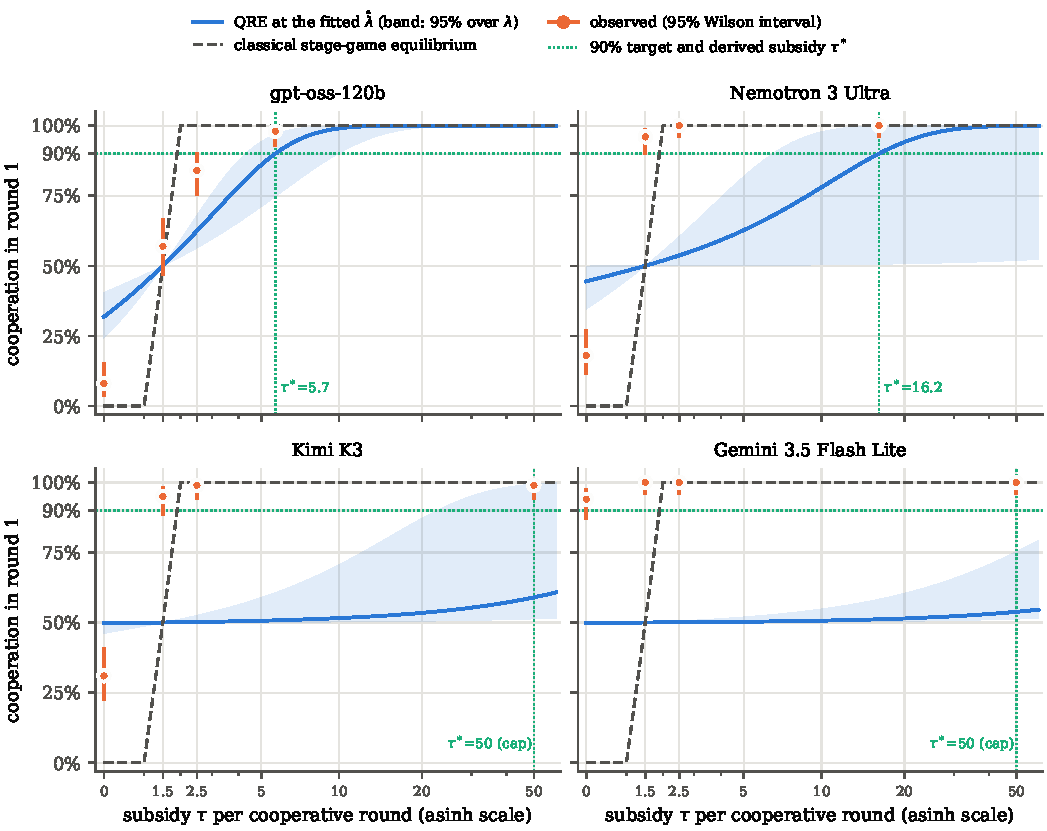
\includegraphics[width=\textwidth]{figures/stage5.pdf}
\caption{Stage 5: round-1 cooperation against the subsidy $\tau$, one panel per model. Orange:
observed rate with 95\% Wilson interval (100 questions per level). Blue: logit QRE at the model's
fitted Stage 2A precision $\hat\lam$ (posterior median), with the 95\% band over $\lam$'s posterior.
Dashed: the classical stage-game equilibrium (all defect below $\tau=1$, the mixed equilibrium
$p=\tau-1$ of the chicken game between 1 and 2, all cooperate above 2). Dotted: the 90\% target
and the derived subsidy $\tau^*$ (capped at 50).}
\label{fig:stage5}
\end{figure}}{}

\begin{table}[t]
\centering
\caption{Stage 5: round-1 cooperation (\%) under the subsidy $\tau$, 100 questions per cell,
against each theory's prediction. QRE is evaluated at the model's fitted Stage 2A precision
$\hat\lam$ (posterior median). Classical is the stage-game equilibrium. The last column is
Stage 2A's identical question without the subsidy rule. $^\dagger$At the registered cap.}
\label{tab:stage5}
\small
\begin{tabular}{@{}lrr cccc c@{}}
\toprule
 & & & \multicolumn{4}{c}{Cooperation at subsidy $\tau$} & No rule \\
\cmidrule(lr){4-7}
Model & $\hat\lam$ & $\tau^*$ & 0 & 1.5 & 2.5 & $\tau^*$ & (2A) \\
\midrule
gpt-oss-120b & 0.579 & 5.7 & 8 & 57 & 84 & 98 & 31 \\
Nemotron 3 Ultra & 0.154 & 16.2 & 18 & 96 & 100 & 100 & 41 \\
Kimi K3 & 0.0075 & 50$^\dagger$ & 31 & 95 & 99 & 99 & 54 \\
Gemini 3.5 Flash Lite & 0.0032 & 50$^\dagger$ & 94 & 100 & 100 & 100 & 91 \\
\midrule
\multicolumn{3}{@{}l}{Classical prediction} & 0 & 50 & 100 & 100 & \\
\multicolumn{3}{@{}l}{QRE prediction, gpt-oss} & 32 & 50 & 62 & 90 & \\
\multicolumn{3}{@{}l}{QRE prediction, Nemotron} & 44 & 50 & 54 & 90 & \\
\multicolumn{3}{@{}l}{QRE prediction, Kimi / Gemini} & 50 & 50 & 50 & 59 / 54 & \\
\bottomrule
\end{tabular}
\end{table}

All 1{,}600 Stage 5 answers were collected after pre-registration~4 was filed (first answer two
minutes after the registration time stamp). Table~\ref{tab:stage5} and
Figure~\ref{fig:stage5} give the results. The four registered tests read as follows.

\paragraph{Test 1: at $\tau=2.5$, classical theory predicts better than QRE, for every model.}
The difference in absolute error (classical minus QRE) is $-46$ points for Nemotron, $-48$ for
Kimi and $-50$ for Gemini, with bootstrap intervals far from zero. For gpt-oss it is $-6$ points
$[-20,+8]$: classical theory is closer, but not decisively. Every model cooperates at least 84\%
once cooperation is dominant, where QRE at the fitted precision predicts 50--62\%.

\paragraph{Test 2: the derived mechanism reaches its target, and overshoots it.} At $\tau^*$,
cooperation is 98--100\% for every model, inside the registered band of $90\pm15$. For every
model, though, the 95\% interval lies wholly above 90\%: the mechanism worked, but it overpaid.
The overpayment is largest where Proposition~\ref{prop:ceiling} predicts it. In Stage~2A,
Gemini cooperated 91\% of the time with no subsidy and Kimi 54\% (the latter not significantly
above one half), so their fitted $\lam$ (0.0032 and 0.0075) sits near the floor of the grid
($10^{-3}$) and $\tau^*$ hits the cap of 50, twenty times the 2.5 at which they already cooperate
99--100\%. Only for gpt-oss did the derived subsidy earn its cost: the classical guess of 2.5
reached 84\%, short of the 90\% target, and $\tau^*=5.7$ reached 98\%.

\paragraph{Test 3: the parameter-free halfway point holds for one model.} Corollary~\ref{cor:half}
predicts exactly 50\% at $\tau=1.5$ for any regular quantal responder. gpt-oss cooperates 57\%
$[47,66]$ (exact binomial $p=0.19$), consistent with the prediction. The other three cooperate
95--100\% (Holm-adjusted $p<10^{-21}$), which by Proposition~\ref{prop:ceiling} no regular QRE
can produce. Cooperation this high at $\tau=1.5$ is consistent with the subgame-perfect
repeated-game cooperation described in Section~\ref{sec:mechanism} and with a cooperation norm;
Stage~5 alone does not separate the two.

\paragraph{Test 4: calibration.} Only 3 of 16 cells are within $\pm10$ points of QRE: gpt-oss at
$\tau=1.5$ and $\tau^*$, and Nemotron at $\tau^*$, where QRE's 90\% and the observed 100\% are
both near the ceiling.

\paragraph{Stating the rule changes play.} The registered comparison of $\tau=0$ with Stage~2A
isolates the effect of merely stating a subsidy rule, with a subsidy of zero. Cooperation falls
for three models: gpt-oss from 31\% to 8\%, Nemotron from 41\% to 18\% and Kimi from 54\% to
31\% (each $p<0.001$). Gemini is unchanged (91\% vs 94\%, $p=0.44$). A payoff rule on the page
seems to move these models from the cooperative script towards the payoff calculation. That is
itself a mechanism-design effect: the framing of an incentive matters even when the incentive is
zero.

\paragraph{Pre-registration~4, scored.} The headline prediction was amended on 3 October 2026,
before three of the four models' Stage~2A fits existed and nine days before the first Stage~5
answer; the original headline (that $\tau^*$ yields more cooperation than 2.5) was dropped as
near-mechanical. The amended prediction was that classical theory would beat QRE at $\tau=2.5$
for Nemotron and Kimi, that $\tau^*$ would overshoot, and
that QRE would be closest only for Gemini. The first two parts held; the third failed, because
classical theory was also closer for Gemini. Our level-by-level forecasts were closer
to the data than either theory for gpt-oss and Kimi (mean absolute error 6.5 and 13 points,
against 8.3 and 19.5 for classical theory and 15.3 and 38.3 for QRE). For Nemotron they were as
close as classical theory (16.5 against 16.0 points). They missed badly for Gemini (43.5 points),
whose near-universal cooperation at $\tau=0$ we did not foresee. This comparison
is descriptive and was not registered.

\paragraph{What Stage 5 shows.} A low fitted $\lam$ suggests agents that barely respond to
incentives. Three of the models do the opposite: gpt-oss, Nemotron and Kimi move from 8--31\%
cooperation with no subsidy to 84--100\% at $\tau=2.5$, far more than QRE at their fitted
precision allows, and Nemotron and Kimi exceed even the classical stage-game prediction at
$\tau=1.5$ (95--96\% against 50\%). The fourth, Gemini, cooperates 94--100\% at every level,
including $\tau=0$: it is a constant cooperator, so Stage~5 does not measure its responsiveness.
In every case the low prisoner's dilemma $\lam$ reflected cooperation on the unsubsidised question
that QRE cannot represent (conditional cooperation, Section~\ref{sec:stage2b}), not noise in
responding to payoffs. A designer who took it at face value would set subsidies up to twenty
times larger than needed.

% =====================================================================================
\section{Discussion}\label{sec:discussion}

\paragraph{``Derive or recall'' has no single answer.} The same question receives different
answers across models and games:
\begin{itemize}
\item Nemotron's and Kimi's Cournot play survives the removal of every cue that could trigger
  recall, and both re-derive the answer when a trap changes one rule;
\item gpt-oss's play degrades step by step as the cues are removed, its errors become the
  cooperative (collusive) answer, and in the traps it gives the textbook answer about five
  times as often in the standard wording;
\item Gemini's Cournot play does not survive the removal of the game's familiar vocabulary;
\item for games whose rules are their fingerprint (the second-price auction, public goods), no
  wording hid the game from the strongest models, so derivation and recall remain observationally
  equivalent there.
\end{itemize}
The last point is a limit of the method, not a failure of it: recognising a game's structure is
itself a form of reasoning. More striking is that our own pre-registered expectations
about \emph{which} models recall were reversed. Intuition about which LLMs ``really reason'' is
unreliable, and that is a reason to measure it.

\paragraph{Competence and robustness (suggestive).} The pre-registered ranking matched: models
that pass more competence probes lose less when the game is disguised. With four models and pass
rates that differ by one to three questions at the top, this is weak evidence. If it holds up
across more models, probe pass rates under paraphrase would be a cheap screen for agents that will
face unfamiliar rules.

\paragraph{Recognition can pull away from equilibrium.} The usual worry is that recall makes
models look more rational than they are. In the prisoner's dilemma we find the reverse.
Recognising the game lowers equilibrium play: Gemini by 62 points under the standard disguise,
and every model by 17--76 points relative to the extreme wording. The retrieved content is conditional cooperation, the folk
lesson of repeated dilemmas (trust, reciprocity), not the backward-induction solution, much as
calling a human prisoner's dilemma the ``Community Game'' raises cooperation
\citep{liberman2004name}. For
mechanism design this matters directly: an agent's behaviour depends on which famous game the
designer's rules resemble.

\paragraph{Probes change conclusions.} Without competence probes, Gemini's disguised auction
would read as a 92-point strategic collapse. With them, it is correctly a reading failure.
Without a registered slip rule, Nemotron's extreme-wording Cournot and auction results would
read as 46- and 51-point drops. Both safeguards altered headline numbers, which is the strongest
argument for building them in before the data.

\paragraph{Implications for designing mechanisms for AI agents.} Theorem~\ref{thm:alpha} gives a
cheap diagnostic: rescale the payment rule and check whether bids rescale. Theorem~\ref{thm:subsidy}
shows that noise makes high compliance expensive, so subsidies should be set from measured
responsiveness rather than from dominance thresholds. And the decision gate warns against borrowing the
behavioural model wholesale. Logit QRE fails held-out calibration for every model, because LLM
errors are rare, large and discrete: slips, collusive answers and norms. A fitted $\lam$ then
encodes a norm or a slip rate rather than noise. Stage~5 shows the cost: a subsidy derived from
the fitted $\lam$ reached its target but overpaid by up to twenty times, while the classical
dominance threshold was enough for three of four models.

\paragraph{When does a fitted behavioural model mislead?} Proposition~\ref{prop:ceiling} gives a
check that needs no new data: if a population cooperates more than half the time where every
regular QRE predicts at most half, the population is outside the model, and any $\lam$ fitted to
it will be pushed towards zero. Three of our four models fail this check in Stage~5 (95--100\%
cooperation at $\tau=1.5$), and Gemini already fails it without any subsidy (91--94\%). The general lesson is that a precision parameter fitted to one
setting (here, the unsubsidised game) can measure something other than responsiveness (here,
cooperation that the model cannot represent), and then extrapolates badly to the setting a
designer cares about. Checking a behavioural model's qualitative restrictions before trusting its
parameters is cheap, and here it would have flagged the overpayment in advance.

\paragraph{Framing is part of the mechanism.} Stating a subsidy rule of zero cut cooperation by
23 points in three models. Framing effects are well documented in people \citep{tversky1981framing}; in the prisoner's
dilemma, merely renaming the game changes human cooperation \citep{liberman2004name}. For LLM
agents, the text of a rule, and not only its payoffs, is a design variable.

% =====================================================================================
\section{Limitations}\label{sec:limitations}

\begin{itemize}
\item \textbf{Disguises can fail.} The standard disguise did not hide the games from two of the four
  models (Nemotron and Kimi), and no wording hid the auction or public goods. Recognition is coded from written
  reasoning, so silent recognition cannot be excluded.
\item \textbf{A leaky answer box.} In Stage~2A's disguised wording the answer field still carried
  the standard wording's field names (``bid'', ``quantity'', ``contribution''). This was found after
  collection, is recorded as deviation~8, and was removed in Stage~2C.
\item \textbf{Timing.} Stage~2C was collected weeks after Stage~2A, and Stage~5 after both, so a
  provider updating a model in between would appear as a difference. This applies to the
  Stage~2C comparison and to Stage~5's comparison of $\tau=0$ with Stage~2A (the framing
  effect of stating the rule).
\item \textbf{The behaviour model.} QRE treats every departure from equilibrium as payoff-scaled
  noise. Our models' departures are often slips or norms instead, so $\lam$ is a summary, not a
  structural parameter \citep{pechon2026auditing}, and it is never compared across games.
\item \textbf{The $\lam$ grid.} The registered grid tops out at $\lam = 1000$, where QRE cannot
  reproduce 100\% equilibrium play in the auction. This affects the calibration of those cells,
  but not the gate's verdict.
\item \textbf{The stage-game QRE in the prisoner's dilemma.} It ignores continuation play, which
  is harmless when the stage equilibrium is unique but not at $\tau=1.5$.
\item \textbf{Stage 5 is one game.} The subsidy test uses the prisoner's dilemma only, with one
  wording, and 100 questions per level. Cooperation above one half at $\tau=1.5$ is consistent
  with both a norm and subgame-perfect repeated-game play, and Stage~5 does not separate them.
\item \textbf{Data collection on NVIDIA's degraded days.} Kimi returned scrambled replies on 7--9
  October 2026; 219 unreadable Stage~2B answers from those days were re-asked at our
  decision (Appendix~\ref{app:deviations}). Only unreadable answers were re-asked, so the re-ask
  is selective; results are reported both ways.
\item \textbf{Scope.} Four models, four games and free API tiers with default sampling.
  Cross-model patterns are rankings, not estimates of population effects.
\end{itemize}

% =====================================================================================
\section{Conclusion}

Whether an LLM agent derives or recalls a game's equilibrium is an empirical property of the
model and the game, and it can be measured. Isomorphic twins with same-wording competence
probes, measured recognition and an extreme disguise separate the two wherever the game can be
hidden at all. On that evidence:
\begin{itemize}
\item two frontier models solve a Cournot game they no longer recognise, and are not fooled by
  traps that make the textbook answer wrong;
\item a third loses the equilibrium step by step as the cues are removed;
\item a fourth loses it as soon as the familiar vocabulary goes;
\item in the prisoner's dilemma, recognising the game pulls every model away from equilibrium,
  towards cooperation, and three of four cooperate early in a repeated game and defect late, as
  people do;
\item the standard behavioural model, logit QRE, does not describe any of them.
\end{itemize}
For mechanism design these are not curiosities. They determine whether a rule tuned to observed
play will survive a change in the rules. In a pre-registered test, a subsidy derived from fitted
quantal response did reach its target, but overpaid by up to twenty times, because the models
respond to incentives more sharply than the fitted model allows. Before designing for AI agents
from a behavioural model, the model itself should be tested on them.

% =====================================================================================
\subsubsection*{Broader Impact Statement}
This work measures how LLM agents behave in strategic settings and tests a mechanism designed for
them; it involves no human participants and no personal data. Its main practical implication is
cautionary: behavioural models fitted to LLM play can mislead a designer (here, a subsidy that
overpays by up to twenty times), and an agent's play can depend on whether a familiar game is
recognised. Both bear on deploying LLM agents in markets and auctions. The traps and disguises
could in principle be used to probe models adversarially; we see this as a benefit for
evaluation rather than a risk.

\subsubsection*{Use of Large Language Models}
An AI assistant (Claude, Anthropic) assisted with code, typesetting and drafting. The research
questions, pre-registered predictions and decisions are the authors', and the authors take full
responsibility for the content.

\subsubsection*{Reproducibility}
Code, prompts, seeds, every raw answer, analysis outputs and the locked analysis plans are provided
in anonymized form as supplementary material and will be made public with the paper.

\bibliographystyle{tmlr}
\bibliography{refs}

\clearpage
\appendix

\section{Example questions}\label{app:prompts}

The questions below are reproduced verbatim from the frozen question code (seed 20260845, first
paraphrase). Each is sent as a single user message, followed by a separate maths check in the
same wording. Figure~\ref{fig:design} shows a Cournot question in all three wordings.

\paragraph{Prisoner's dilemma, standard wording (Stage 2A).}
{\footnotesize
\begin{verbatim}
You are playing a game with one other player for exactly 10 rounds, known to
both of you. Each round you both simultaneously choose C or D.
  If you both choose C, you each score 3.0.
  If you both choose D, you each score 1.0.
  If you choose D and they choose C, you score 5.0 and they score 0.0.
  If you choose C and they choose D, you score 0.0 and they score 5.0.
This is round 1. History so far: none yet
Choose C or D.
\end{verbatim}}
\noindent\emph{Maths check:}\nopagebreak
{\footnotesize
\begin{verbatim}
Two players simultaneously choose C or D. Your own score:
  you choose C, they choose C  ->  you score 3
  you choose D, they choose C  ->  you score 5
  you choose C, they choose D  ->  you score 0
  you choose D, they choose D  ->  you score 1
Consider ONE round in isolation. They choose C. Which of your two choices scores
you more? Reply with the single letter only.
\end{verbatim}}

\paragraph{The same question, disguised wording (Stage 2A).}
{\footnotesize
\begin{verbatim}
You and one other technician each operate a control panel for a session of
exactly 10 rounds, known to both of you. Each round, you both simultaneously
set your panel to position Y or position X.
   If you both set Y, you each receive 3.0 units.
   If you both set X, you each receive 1.0 units.
   If you set X and they set Y, you receive 5.0 units and they receive 0.0.
   If you set Y and they set X, you receive 0.0 units and they receive 5.0.
This is round 1. History so far: none yet
Set your panel to Y or X.
\end{verbatim}}
\noindent\emph{Maths check:}\nopagebreak
{\footnotesize
\begin{verbatim}
Two technicians simultaneously set panels to position Y or X. Your own units
received:
  you set Y, they set Y  ->  you receive 3
  you set X, they set Y  ->  you receive 5
  you set Y, they set X  ->  you receive 0
  you set X, they set X  ->  you receive 1
Consider ONE round in isolation. They set Y. Which of your two settings gives
you more? Reply with the single letter only.
\end{verbatim}}

\paragraph{The double-payment trap, standard wording (Stage 2B).} The correct bid is half the
value; the textbook answer, bidding the value, loses money whenever the second bid exceeds half
the value.
{\footnotesize
\begin{verbatim}
You are bidding in a sealed-bid auction for a single item against 2 other
bidders. The highest bidder wins and pays TWICE the SECOND-highest bid
submitted. Your private value for the item is 75.6 tokens -- winning at a
price below that value profits you the difference, and winning above it
loses you the difference. Submit your bid.
\end{verbatim}}
\noindent\emph{Maths check} (answer: $50-2\times20=10$; the single-payment answer is 30):\nopagebreak
{\footnotesize
\begin{verbatim}
In a sealed-bid auction the highest bidder wins and pays TWICE the
SECOND-highest bid submitted. Your private value is 50 and you bid 40. The
highest bid among the other bidders is 20. What is your payoff?
\end{verbatim}}

\paragraph{The subsidy question (Stage 5, $\tau=2.5$).} The subsidy is stated as a separate rule,
so the payoff table is identical to Stage~2A's.
{\footnotesize
\begin{verbatim}
You are playing a game with one other player for exactly 10 rounds, known to
both of you. Each round you both simultaneously choose C or D.
  If you both choose C, you each score 3.0.
  If you both choose D, you each score 1.0.
  If you choose D and they choose C, you score 5.0 and they score 0.0.
  If you choose C and they choose D, you score 0.0 and they score 5.0.
On top of these scores, each player is paid an extra 2.5 points in every round
in which that player chooses C.
This is round 1. History so far: none yet
Choose C or D.
\end{verbatim}}

\section{Deviations from the pre-registrations}\label{app:deviations}
\begin{enumerate}
\item \textbf{PD scoring error in practice runs.} Standard-wording answers were scored against the disguised
  labels; fixed before Stage~2.
\item \textbf{Gemini~3.8~Flash replaced} by Gemini~3.5~Flash~Lite, because of a 20-request
  daily cap.
\item \textbf{Empty replies} (bursts of ``!!!!'') are re-asked rather than scored as unreadable.
\item \textbf{gpt-oss's daily token cap} slows its collection; this does not affect the design.
\item \textbf{A 10-minute NVIDIA access outage.} Its 4{,}454 refused requests were relabelled as
  infrastructure failures and re-asked.
\item \textbf{The fraction slip.} Recorded as an exploratory observation, and corrected only in
  the pre-registration-3 comparison.
\item \textbf{Block~D (reasoning effort)} was dropped before any of its data existed, so that all
  models answer the same questions.
\item \textbf{The disguised answer boxes} carried the standard wording's field names (a limitation).
\item \textbf{Ten questions re-asked} that should have been scored as the model's own (1 Kimi
  Stage~2A; 2 Nemotron Stage~2A; 7 Nemotron Stage~2B traps). The re-asked answers stand.
\item \textbf{The pilot answer form} sent explanatory text that leaked words; fixed before
  Stage~2C.
\item \textbf{A second provider for gpt-oss} (Cerebras, same open weights) was recorded as an option
  for Stage~2B and never used. Every gpt-oss answer comes from Groq.
\item \textbf{Additional API keys.} A second Gemini key and three further Groq keys, each from a
  different person's account, were used after the providers' support teams confirmed in writing
  that this is permitted. Same models and settings. Remaining work was split into disjoint
  slices of the registered question list, so no question was asked twice.
\item \textbf{One NVIDIA refusal} (``DEGRADED function cannot be invoked'') had been scored as an
  unreadable Kimi answer; it was relabelled a server refusal and re-asked.
\item \textbf{Kimi's unreadable answers from NVIDIA's degraded days} (7--9 October 2026) were
  re-asked at our decision: 219 answers, 16\% of that window against about 3\% on other
  days. Only unreadable answers were re-asked; the originals remain in the data, and affected
  results are reported both ways.
\end{enumerate}

\section{Stage 2A precision fits}\label{app:lambda}

\begin{table}[h]
\centering
\caption{Posterior $\lam$ for Stage~2A (median and 95\% interval), standard vs disguised wording.
$\lam$ is on each game's payoff scale and is not comparable across games. The grid is
log-uniform on $[10^{-3},10^{3}]$. A cell with more than 5\% of its posterior mass in the top
5\% of the log grid is a \emph{ceiling} cell: only a lower bound is identified, and ``$\ge$''
reports the posterior 2.5\% quantile. A cell with more than 5\% of its mass in the bottom 5\% is a
\emph{floor} cell: ``$\le$'' reports the 97.5\% quantile, with the median in parentheses.}
\label{tab:lambda}
\small
\begin{tabular}{@{}lllll@{}}
\toprule
Model & Game & $\lam$ standard & $\lam$ disguised & $\Delta\lam$ \\
\midrule
gpt-oss & Vickrey & $\ge944$ & 1.12 $[0.87,1.45]$ & $\ge+943$ \\
 & Cournot & 0.173 $[0.13,0.22]$ & 0.027 $[0.022,0.035]$ & $+0.146$, $P(>0)=1.00$ \\
 & PD & 0.579 $[0.27,0.92]$ & 0.772 $[0.45,1.12]$ & $-0.19$, $P(>0)=0.20$ \\
 & Public goods & 3.76 $[3.07,4.34]$ & 1.19 $[1.00,1.37]$ & $+2.53$, $P(>0)=1.00$ \\
Nemotron & Vickrey & $\ge944$ & $\ge944$ & both at ceiling \\
 & Cournot & $\le0.0015$ (0.0012) & $\le0.0012$ (0.0010) & $+0.0001$, $P(>0)=0.82$ \\
 & PD & 0.154 $[0.002,0.47]$ & 0.188 $[0.002,0.50]$ & $-0.02$, $P(>0)=0.44$ \\
 & Public goods & $\ge21.8$ & $\ge21.8$ & both at ceiling \\
Kimi & Vickrey & $\ge944$ & $\ge944$ & both at ceiling \\
 & Cournot & $\ge299$ & 19.4 $[14.1,26.6]$ & $\ge+272$ \\
 & PD & $\le0.11$ (0.0075) & $\le0.39$ (0.079) & $-0.06$, $P(>0)=0.21$ \\
 & Public goods & 2.51 $[2.11,2.90]$ & 3.98 $[3.35,4.73]$ & $-1.51$, $P(>0)=0.00$ \\
Gemini & Vickrey & $\ge944$ & 3.98 $[1.5,7.7]$ ($n=11$) & $\ge+936$ \\
 & Cournot & 0.649 $[0.50,0.82]$ & 0.0047 $[0.0036,0.0060]$ & $+0.645$, $P(>0)=1.00$ \\
 & PD & $\le0.023$ (0.0032) & 0.631 $[0.33,0.97]$ & $-0.629$, $P(>0)=0.00$ \\
 & Public goods & $\ge21.8$ & 0.434 $[0.36,0.53]$ & $\ge+21.2$ \\
\bottomrule
\end{tabular}
\end{table}

\noindent Nemotron's Stage~2A Cournot fit is dominated by uncorrected fraction slips (answers
such as 683 for $683/60$), which are scored as they were written, as pre-registration~1
requires; this is what puts it at the floor. With the slip correction fixed in
pre-registration~3, its standard-wording Cournot $\lam$ is 0.0082 $[0.0063,0.0103]$ (Stage~2C
analysis output, \texttt{results/analysis/stage2c\_nemotron.md}). Kimi's Cournot difference
arises entirely within the $\pm0.5$ tolerance: both wordings are at 100\% equilibrium play. Stage~5
uses the posterior medians of the standard-wording prisoner's dilemma cells; for Kimi and Gemini
these are floor cells, so their $\tau^*$ is set by the registered cap.

\end{document}
